\section{PTC thermistors}
As aforementioned, a positive temperature coefficient thermistor (also called \textbf{posistor}) is a thermally sensitive resistor that varies its resistivity as the temperature of the environment changes. Particularly because it is a positive coefficient, as the temperature increases, the resistivity of the semiconductor device increases as well.

The posistor's structure is rather simple: a PTC material is put between two metal foil electrodes. The overall resistance of the PTC thermistor is given by the PTC material (also called \textsl{bulk}), the electrode resistance (which can be omitted) and the interface resistance \cite{Tang2023}. 

\subsection{Charateristics}
One of the most important properties of the PTC thermistor is the characteristic curve between the \textbf{resistance} $R$ and the \textbf{temperature} $T$, which has to be converted from Celsius (or Fahrenheit) to Kelvin. Its curve is a positive exponential graph that respects the following equation \cite{Saburi196353}\cite{jones2010biomedical}:

\begin{equation*}
    R = R_0\,e^{\beta\,(\frac{1}{T} - \frac{1}{T_0})}
\end{equation*}

\noindent Where $R$ is the calculated resistance at the temperature $T$ and $R_0$ is the resistance measured at temperature $T_0$. The coefficient $\beta$ is the thermistor constant and it depends on the materials used to build it and on the thermistor dimensions. It is possible to obtain this value by measuring its resistance value at two different temperatures and computing the following equation \cite{Saburi196353}.

\begin{equation*}
    \beta = \frac{\ln{\frac{R_2}{R_1}}}{\frac{1}{T_2} - \frac{1}{T_1}}
\end{equation*}

\noindent Using the previous equations, the curve can be plotted by writing down the equations using MATLAB, or other programming languages. Figure \ref{fig:PTC_logarithmic} shows how much the resistance increases as the temperature increases. In this case, the coefficient $\beta$ has been calculated by assuming that when $T_1 = 273.15 K$, $R_1 = 1k\Omega$ and when $T_2 = 373.15 K$, $R_2 = 100M\Omega$.\footnote{Please be aware that the selected values are purely for illustrative purposes; no devices with these characteristics exist in reality}

\begin{figure}[h]
    \centering
    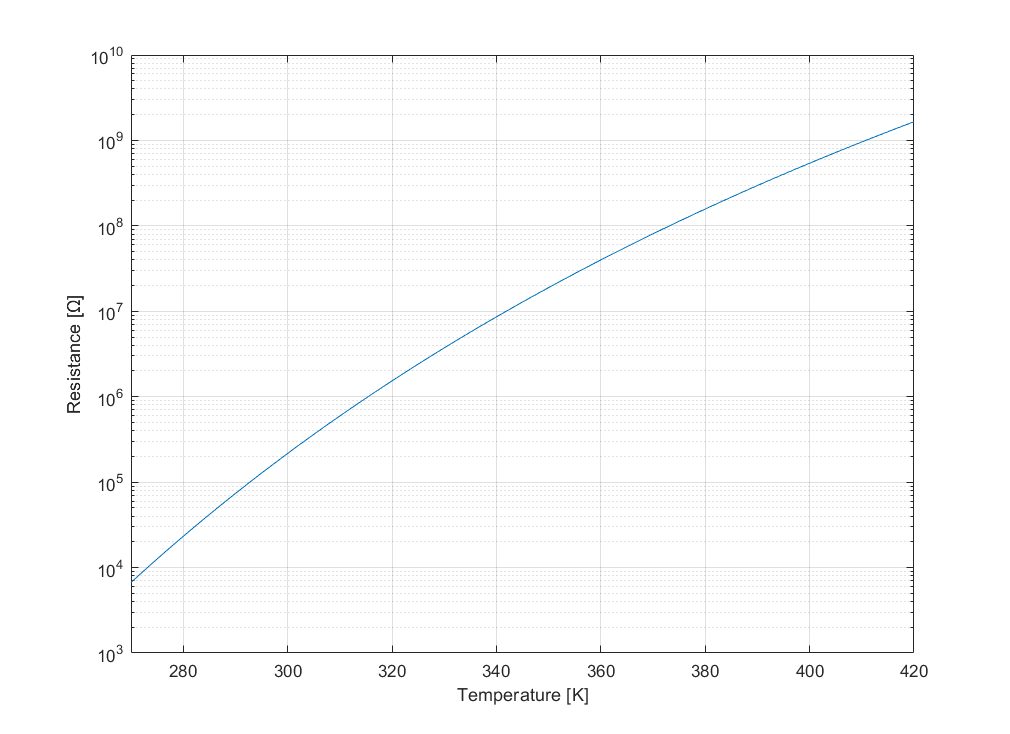
\includegraphics[width = .75\textwidth]{../res/plots/PTC_logarithmic.png}
    \label{fig:PTC_logarithmic}
    \caption{PTC resistance-temperature logarithmic curve.}
\end{figure}

\FloatBarrier\noindent Secondly it might be interesting to plot the change ratio between the resistance $R$ and the value of the resistance at some fixed temperature. In the figure \ref{fig:PTC_ratio}, the fixed temperature value $T_0$ was 25° celsius (or 298.15 Kelvin) which implies that $R_0 = 16.7 k\Omega$.

\begin{figure}[h]
    \centering
    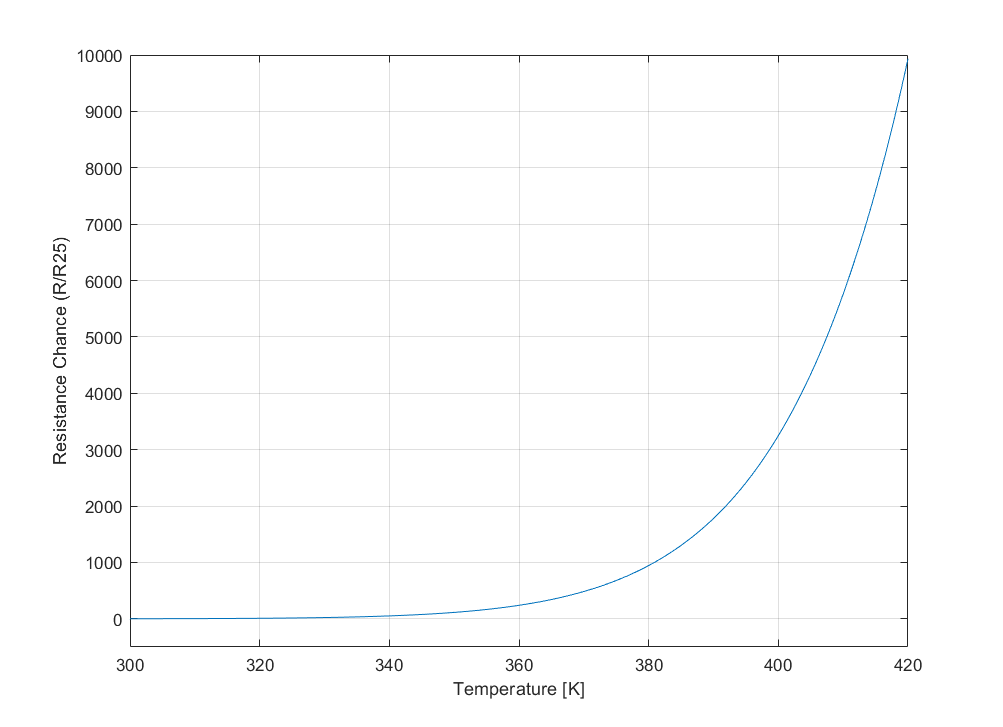
\includegraphics[width = .75\textwidth]{../res/plots/PTC_ratio.png}
    \label{fig:PTC_ratio}
    \caption{PTC change ratio between $R$ and $R_0$}
\end{figure}

\FloatBarrier\noindent In both of the plots the resistance value or the change ratio drastically increases as the environment gets hotter. Generally, the equation describes the behavior of the PTC thermistor in an interval of temperature: in the PTC materials there is a temperature, called \textbf{Curie point} where the resistance starts to rise exponentially in comparison with the temperature (as shown in figure \ref{fig:PTC_logarithmic} and \ref{fig:PTC_ratio}); before the Curie temperature, the PTC thermistor does not increase drastically their resistance when the temperature raises. Generally, the Curie point in the PTC materials is between 50°C and 400°C \cite{Cheng2014441}.

Another important coefficient to know about is the \textbf{dissipation constant} $\delta$ which describes the power needed to increase the thermistor temperature by 1° Celsius through self-heating. The dissipation constant varies on the construction materials of the thermistor and the environment \cite{Saburi196353}. The constant $\delta$ is useful to describe the power dissipation of the thermistor when its temperature is $T$ (at thermal equilibrium) and the ambient temperature is $T_0$:

\begin{equation*}
    P = VI = \delta(T - T_0)
\end{equation*}

\noindent By knowing the power dissipation it is then possible to plot the \textbf{current-voltage} relationship when the PTC thermistor is in a state of thermal equilibrium. Sure enough, by knowing the constant $\delta$ and the room temperature $T_0$, the power dissipation $P$ can be obtained and then it is possible to calculate the voltage and the current relationship:

\begin{equation*}
    V = \sqrt{P \cdot R} \hspace{50px} I = \sqrt{\frac{P}{R}}
\end{equation*}

\noindent By setting $\delta = 4.5 mW/^{\circ}C$ and the room temperature $T_0 = 25^{\circ}C = 298.15^{\circ} K$, it is possible to plot some important relationship. Figure \ref{fig:PTC_curr-temp} describes the relationship between the current and the temperature in the PTC thermistor: as the temperature increases the current decreases; this is because when the temperature increases, also the resistance increases and, as such, the current flowing through will reasonably decrease.

\begin{figure}[h]
    \centering
    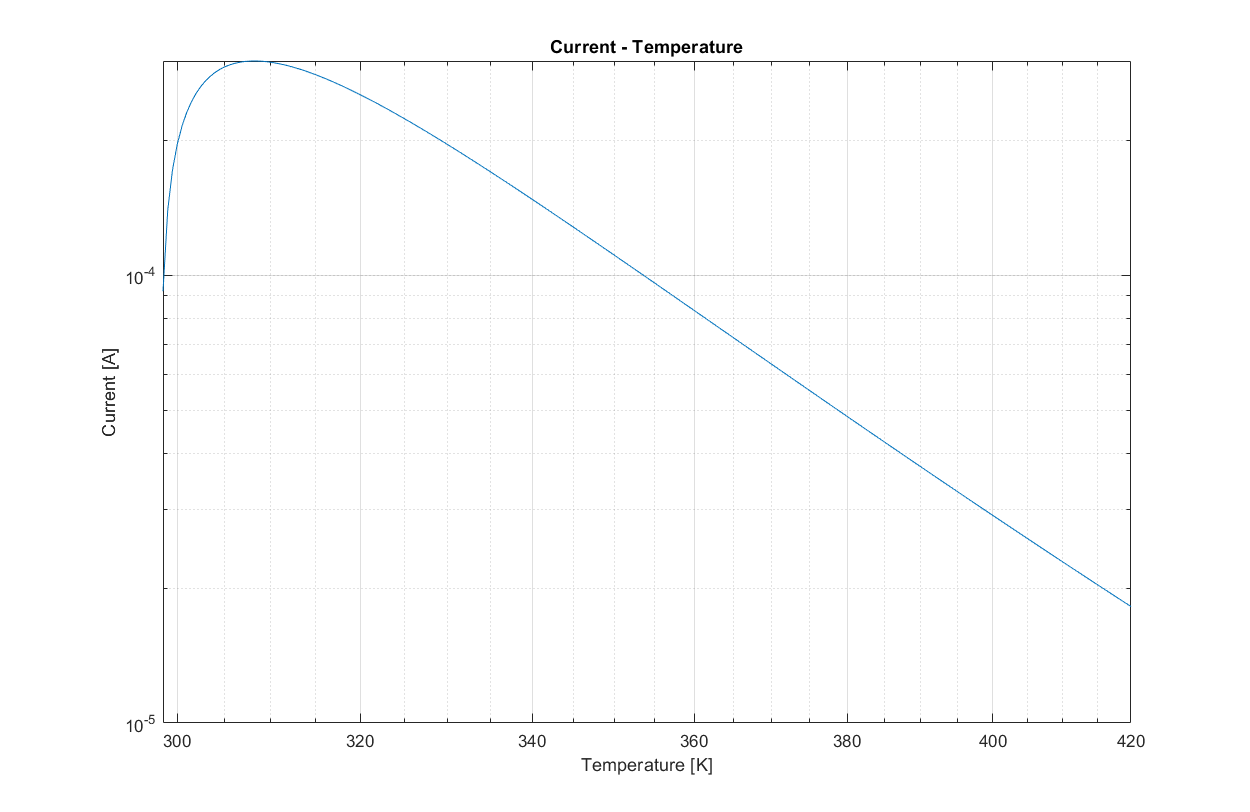
\includegraphics[width = .75\textwidth]{../res/plots/PTC_curr-temp.png}
    \label{fig:PTC_curr-temp}
    \caption{Corrent-temperature relationship of a PTC thermistor.}
\end{figure}

\FloatBarrier \noindent The relationship between the temperature and the voltage is shown in the image \ref{fig:PTC_volt-temp}. Contrarily to the current-temperature relationship, here, as the temperature increases, the voltage of the thermistor rises as well because its resistivity intensifies.

\begin{figure}[h]
    \centering
    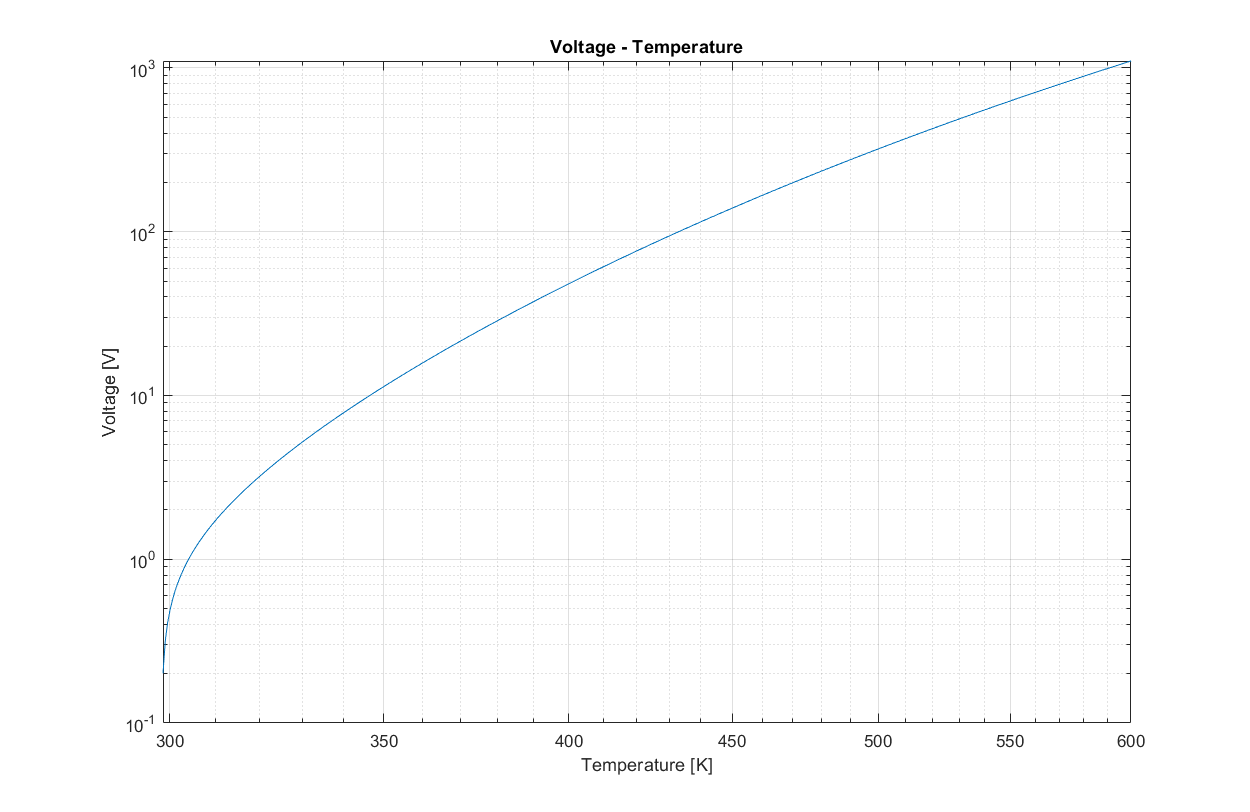
\includegraphics[width = .75\textwidth]{../res/plots/PTC_volt-temp.png}
    \label{fig:PTC_volt-temp}
    \caption{Voltage-temperature relationship of a PTC thermistor.}
\end{figure}

\FloatBarrier \noindent In the figure \ref{fig:PTC_curr-volt} there is the characteristic curve current-voltage of the PTC thermistor. The plot is an \textsl{insofar} curve: when the slope is positive there is a constant-resistance state meanwhile when the slope of the curve is negative there is a constant-power range \cite{Saburi196353}.

\begin{figure}[h]
    \centering
    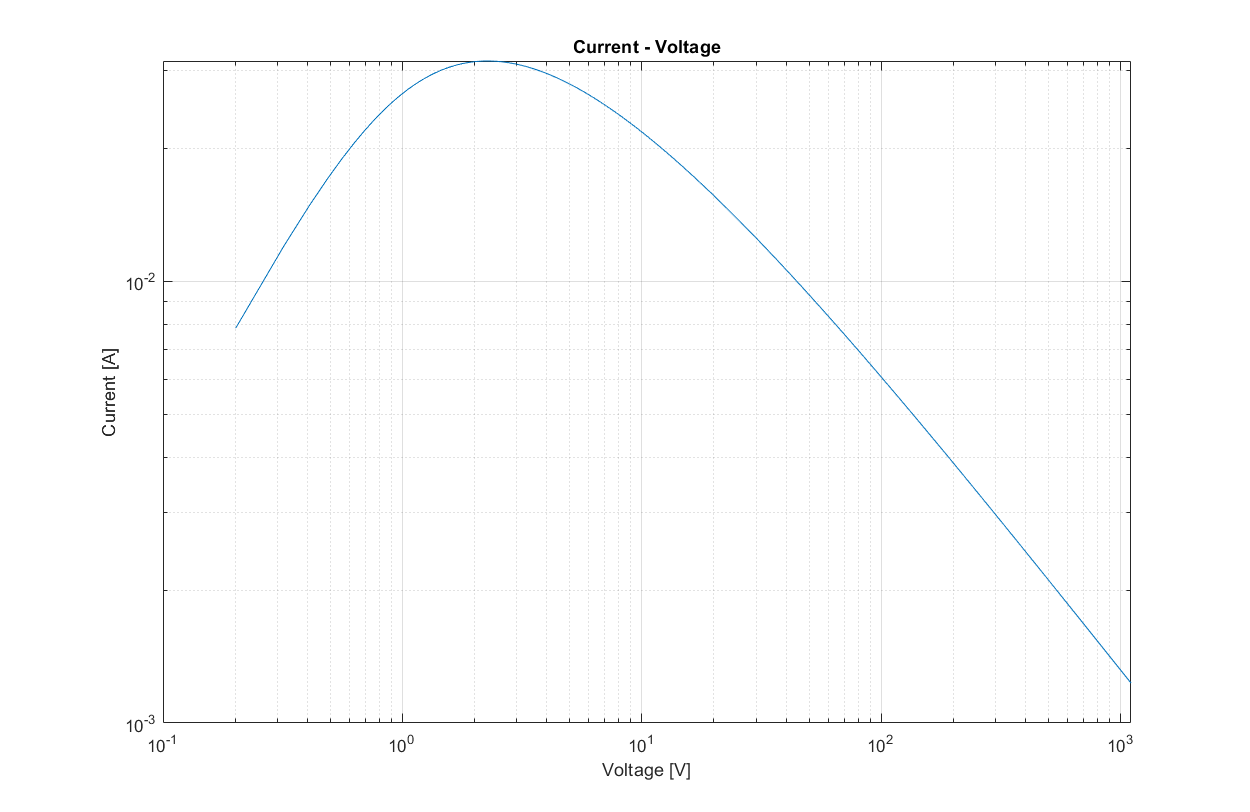
\includegraphics[width = .75\textwidth]{../res/plots/PTC_curr-volt.png}
    \label{fig:PTC_curr-volt}
    \caption{Current-voltage relationship of a PTC thermistor.}
\end{figure}

\FloatBarrier \subsection{Applications}
The applications of the posistors are remarkably important. One of the most popular uses of these devices is as \textit{current limiters} to protect other devices. Sure enough, when there is an excess of current through a circuit it may result in a damaged component of the circuit, like the LED in figure \ref{fig:PTC-circuit-LED}; using a PTC thermistor prevents this from happening because when the current starts increasing through the thermistor, it will heat it making the resistance increase. When the resistance starts increasing the current flowing through it will decrease (as shown in figure \ref{fig:PTC_curr-temp}) and the LED will be protected \cite{Saburi196353}\cite{Perkins1982225}.

\begin{figure}
    \centering
    \begin{circuitikz}[scale = 0.8]
    % Voltage generator
    \draw (0,0) to[V, v=$V$, invert] (0,2);
    
    % Resistance
    \draw (0,2) to[R, l=$R$] (2,2);
    
    % PTC thermistor
    \draw (2,2) to[thR, l=PTC] (4,2);
    
    % LED
    \draw (4,2) to[leD*, l=LED] (4,0);
    
    % Ground
    \draw (4,0) -- (0,0);
\end{circuitikz}
    \label{fig:PTC-circuit-LED}
    \caption{Current limiter PTC application}
\end{figure}

Other important applications are for the \textit{temperature indicator}, when operating in parallel with a diode, or for \textit{temperature control} purposes. In this case, the PTC posistor can control the power dissipated by another device that is connected in series \cite{Saburi196353}\cite{Perkins1982225}. The positive temperature coefficient thermistor may be also utilized to \textit{measure the heating} consumption by a system. For example, it may be used to determine the fuel consumption in a vehicle or the heating consumption in a hot-water-based heating system \cite{Dostert1982159}.

